\newpage
\section{Server}
\subsection{Operazioni Server}
\begin{itemize}
	\item Inizializza una socket \textbf{listenfd} \ref{lst:cass}
	\item Dichiara Insieme di \textbf{Descrittori} \ref{lst:cd}
	\item Seleziona \textbf{Descrittore} \ref{lst:cds}
	\item Verifica ed Utilizza \textbf{Descrittore} \ref{lst:caslss}
	\item Aggiunge Prenotazione 
	\begin{lstlisting}[caption=Codice Query Aggiungi Prenotazione, label=lst:cqap-1]
	read(connfd, &id, sizeof(id));
	read(connfd, &mat, sizeof(mat));
	
	char query_verifica_prenotazione[500];
	
	snprintf(query_verifica_prenotazione, sizeof(query_verifica_prenotazione),
	"select a.id_esame, MIN(data_appello) "
	"from appello a "
	"join esame e "
	"join studente s "
	"where a.id_esame = %d "
	"and data_appello > sysdate() "
	"and anno_corso_studente >= e.anno_corso_esame "
	"and s.mat_studente = '%d' "
	"and (select count(*) from supera s where s.mat_studente = '%d' and s.id_esame = %d) = 0 "
	"group by a.id_esame;", id, mat, id, mat);
	
	if (mysql_query(conn, query_verifica_prenotazione) != 0) {
		fprintf(stderr, "\nmysql_query(query_verifica_prenotazione): %s\n", mysql_error(conn));
		write(connfd, mysql_error(conn), strlen(mysql_error(conn)));
	}
	
	MYSQL_RES *res_qvp = mysql_store_result(conn);
	if (res_qvp == NULL) {		
	\end{lstlisting}
	\begin{lstlisting}[caption=Codice Query Aggiungi Prenotazione, label=lst:cqap-2]
		fprintf(stderr, "\nmysql_store_result(query_verifica_prenotazione): %s\n", mysql_error(conn));
		write(connfd, mysql_error(conn), strlen(mysql_error(conn)));
		}
		
		unsigned int rows = mysql_num_rows(res_qvp);
		/***
		* Se non esiste un appello con questo id e questa data allora restituisco un errore
		*/
		if (!rows) {
		const char *err = "invalid id or data!";
		write(connfd, err, strlen(err));
		} else {
		MYSQL_ROW row_qvp = mysql_fetch_row(res_qvp);
		int id_esame = strtol(row_qvp[0], NULL, 10);
		char data_appello[12];
		strcpy(data_appello, row_qvp[1]);
		
		char inserimento[255];
		snprintf(inserimento, sizeof(inserimento),
		"insert into prenota (mat_studente, id_esame, data_prenotazone) VALUES ('%d', %d, sysdate());",
		mat, id_esame);
		if (mysql_query(conn, inserimento) != 0) {
			write(connfd, mysql_error(conn), strlen(mysql_error(conn)));
		} else {
			char res[255];
			snprintf(res, sizeof(res),
			printf("ttok");
			write(connfd, res, strlen(res));
		}
		}		
	\end{lstlisting}
	\newpage
	\item \textbf{Schema Database}\\
	\subitem
	\begin{figure}
		\begin{center}
		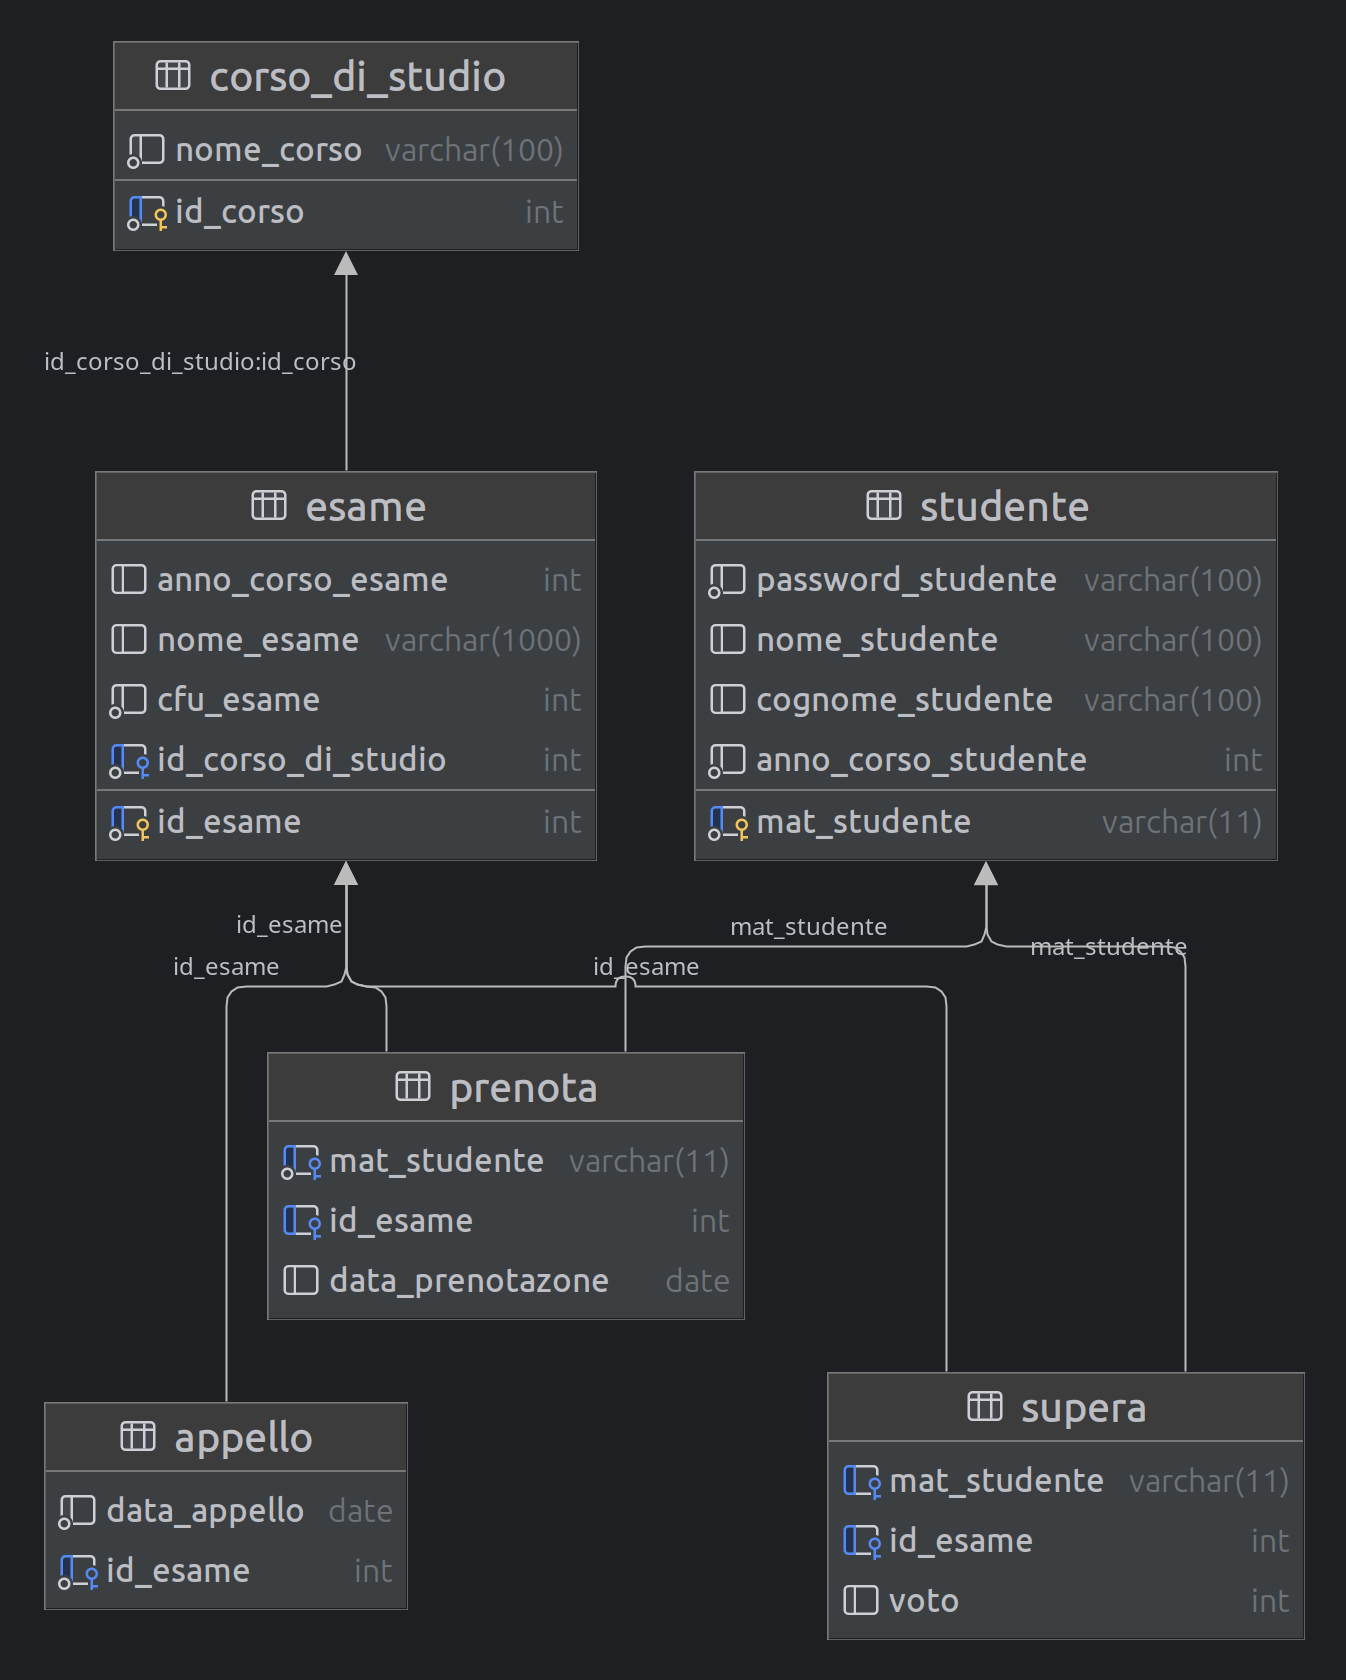
\includegraphics[width=0.7\textwidth]{universitaDB.png}
		\caption{Schema Database Univerisità}
		\label{fig:sdu}
		\end{center}
	\end{figure}
	
			
		

	
\end{itemize}
